\documentclass[../Matt_Gebert_Honours_Thesis.tex]{subfiles}
\begin{document}
	
%	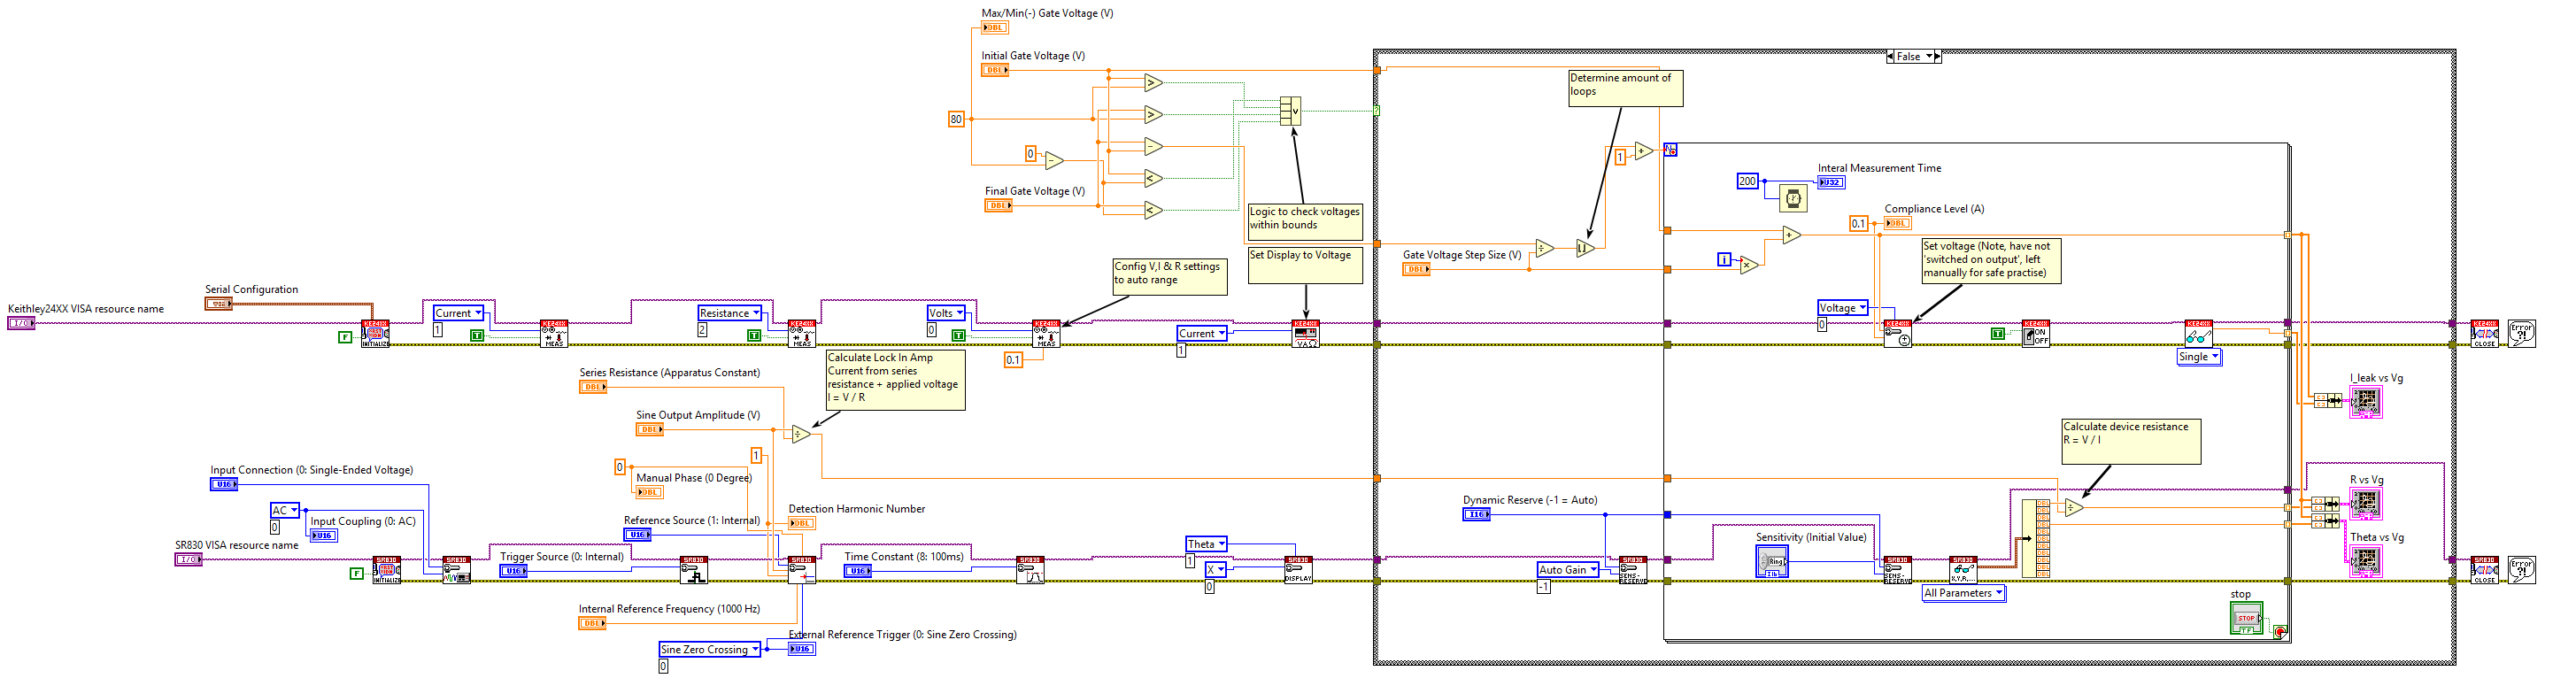
\includegraphics[width=\textwidth]{001_labview.png}
%	In \cref{chap:introduction}, I will outline what I hope to achieve in this project. I begin by discussing the theoretical properties of graphene and why it has attracted so much interest as an electronic material. I will also describe some challenges facing new computing technologies, including the use of dielectrics, and how my work contributes to realising solutions to new generations of this technology. I will outline a theoretical and experimental summary of the results to date seen in introducing dielectrics to graphene.

	\section{Preface}
	
	\section{Transistors - the field effect}
	
	\section{Graphene}
	\subsection{Electronic properties}
	Why is it a good conductor?
	\subsubsection{Hybridisation}
	\subsubsection{Electronic dispersion}
	\subsubsection{Charged puddling}
	
	\section{Transport and scattering in graphene}
	\subsection{Charged impurities}
	\subsection{Dielectric screening}
	\subsubsection{Charge screening}
	\subsubsection{Fine structure constant}
	\subsubsection{}
	\subsection{Phonon scattering}
	\subsection{}
	
	\section{}
	
	
	
\end{document}